\chapter{Cálculo integral}
\label{ch:integral}

En el capítulo anterior estudiamos la derivada como herramienta para describir una tasa instantánea de cambio. El cálculo integral aborda, en cierto sentido, el problema inverso: a partir de una tasa de variación, reconstruir una magnitud acumulada. Si conocemos la velocidad de un móvil, podemos recuperar su desplazamiento; si conocemos el caudal que atraviesa una conducción, podemos calcular el volumen transportado; si conocemos la intensidad de corriente, podemos determinar la carga que ha circulado; y si conocemos una densidad lineal, podemos obtener la masa total de una pieza.

Esta relación entre \emph{tasa} y \emph{acumulación} constituye una de las ideas centrales del cálculo. La integral aparece también al medir áreas, volúmenes y otras magnitudes geométricas. El Teorema Fundamental del Cálculo establece que ambos puntos de vista están íntimamente ligados con la derivación.

\section{Primitivas e integral indefinida}
\label{sec:primitivas}

\subsection{Primitivas y reglas básicas}

Comenzamos con el problema inverso de la derivación. Conocida una función $f$, buscamos una función cuya derivada sea precisamente $f$.

\begin{definition}[Primitiva]
Sea $f:I\to\R$ una función definida en un intervalo $I$. Una función $F:I\to\R$ se llama \emph{primitiva} o \emph{antiderivada} de $f$ en $I$ si
\[
F'(x)=f(x),\qquad \forall x\in I.
\]
\end{definition}

Por ejemplo,
\[
F(x)=x^3
\]
es una primitiva de $f(x)=3x^2$. También lo son $x^3+4$, $x^3-\pi$ o, en general, $x^3+C$ para cualquier constante real $C$.

\begin{theorem}
Si $F$ es una primitiva de $f$ en un intervalo $I$, entonces todas las primitivas de $f$ en $I$ son de la forma
\[
F(x)+C,\qquad C\in\R.
\]
\end{theorem}

\begin{proof}
Si $G$ es otra primitiva de $f$, entonces
\[
(G-F)'=G'-F'=f-f=0.
\]
Por tanto, $G-F$ es constante en $I$, es decir, $G(x)=F(x)+C$.
\end{proof}

\begin{definition}[Integral indefinida]
El conjunto de todas las primitivas de una función $f$ se denomina \emph{integral indefinida} de $f$ y se escribe
\[
\int f(x)\,dx=F(x)+C,
\]
donde $F'(x)=f(x)$ y $C\in\R$ es la \emph{constante de integración}.
\end{definition}

La integral indefinida no es, por tanto, una única función, sino una familia de funciones que difieren en una constante.

La derivación y la integración indefinida son operaciones inversas en el sentido de que
\[
\frac{d}{dx}\left(\int f(x)\,dx\right)=f(x)
\]
y
\[
\int F'(x)\,dx=F(x)+C.
\]

De las reglas de derivación se obtienen inmediatamente reglas de integración. Si $\alpha,\beta\in\R$ y $f,g$ admiten primitivas, entonces
\[
\int \bigl(\alpha f(x)+\beta g(x)\bigr)\,dx
=
\alpha\int f(x)\,dx+\beta\int g(x)\,dx.
\]

Entre las primitivas elementales que utilizaremos con mayor frecuencia están
\[
\int x^n\,dx=\frac{x^{n+1}}{n+1}+C,\qquad n\neq-1,
\]
\[
\int \frac1x\,dx=\ln|x|+C,
\]
\[
\int e^x\,dx=e^x+C,
\qquad
\int a^x\,dx=\frac{a^x}{\ln a}+C\quad (a>0,\ a\neq1),
\]
\[
\int \cos x\,dx=\sin x+C,
\qquad
\int \sin x\,dx=-\cos x+C,
\]
\[
\int \frac{1}{1+x^2}\,dx=\arctan x+C,
\qquad
\int \frac{1}{\sqrt{1-x^2}}\,dx=\arcsin x+C.
\]

Estas fórmulas deben entenderse en intervalos donde las expresiones estén definidas. Por ejemplo, la derivada de $\ln|x|$ es $1/x$ tanto para $x>0$ como para $x<0$.

\begin{example}
Calcular
\[
\int \left(4x^3-\frac{3}{x^2}+2e^x\right)dx.
\]
Aplicando linealidad,
\[
\int4x^3\,dx=x^4,
\qquad
\int -3x^{-2}\,dx=\frac{3}{x},
\qquad
\int2e^x\,dx=2e^x.
\]
Por tanto,
\[
\boxed{\int \left(4x^3-\frac{3}{x^2}+2e^x\right)dx
=x^4+\frac3x+2e^x+C.}
\]
Una comprobación inmediata consiste en derivar el resultado.
\end{example}

\begin{solvedexercise}
La velocidad de un carro que se desplaza sobre una guía es
\[
v(t)=6t^2-4t+3\qquad (\mathrm{m/s}).
\]
Sabiendo que $s(0)=5$ m, determinar su posición $s(t)$.
\tcblower
\textbf{Resolución.}\par\smallskip
Como $s'(t)=v(t)$,
\[
s(t)=\int(6t^2-4t+3)\,dt
=2t^3-2t^2+3t+C.
\]
La condición inicial permite determinar la constante:
\[
5=s(0)=C.
\]
Por tanto,
\[
\boxed{s(t)=2t^3-2t^2+3t+5.}
\]
La constante de integración no es un detalle algebraico: contiene la información sobre la posición inicial, que la velocidad por sí sola no determina.
\end{solvedexercise}

\subsection{De una tasa a una cantidad acumulada}

En muchos modelos de ingeniería no se conoce directamente una cantidad $Q(t)$, sino su tasa de cambio $Q'(t)$. La integración permite reconstruir $Q$ salvo una constante, que debe determinarse mediante una condición inicial.

Si
\[
Q'(t)=r(t),
\]
entonces
\[
Q(t)=\int r(t)\,dt=R(t)+C,
\]
donde $R$ es una primitiva de $r$. La interpretación depende del contexto:

\begin{itemize}
\item si $Q$ es posición, $r$ es velocidad;
\item si $Q$ es carga eléctrica, $r$ es intensidad de corriente;
\item si $Q$ es volumen almacenado, $r$ es caudal neto;
\item si $Q$ es masa producida, $r$ es tasa de producción;
\item si $Q$ es energía transferida, $r$ puede ser una potencia.
\end{itemize}

\begin{example}[Producción acumulada]
Una línea de producción trabaja, durante un cierto régimen, a una tasa
\[
r(t)=40+2t-\frac15t^2
\]
toneladas por hora, donde $t$ se mide en horas desde el inicio del turno. Si $Q(t)$ es la producción acumulada y $Q(0)=0$, entonces
\[
Q'(t)=r(t)
\]
y, por tanto,
\[
Q(t)=40t+t^2-\frac1{15}t^3+C.
\]
Como $Q(0)=0$, resulta $C=0$ y
\[
\boxed{Q(t)=40t+t^2-\frac1{15}t^3.}
\]
Obsérvese la diferencia entre ambas magnitudes: $r(t)$ se mide en toneladas por hora y $Q(t)$ en toneladas.
\end{example}

\section{Métodos de integración}
\label{sec:metodos-integracion}

Las fórmulas inmediatas permiten integrar funciones sencillas. Sin embargo, en la mayoría de los problemas es necesario transformar el integrando hasta reconocer una forma conocida. No existe un algoritmo elemental único que resuelva todas las integrales. Por ello resulta esencial identificar la estructura de la función y elegir el método adecuado.

\subsection{Cambio de variable e integración por partes}

\subsubsection{Cambio de variable}

La regla de la cadena para derivadas afirma que
\[
\frac{d}{dx}F(g(x))=F'(g(x))g'(x).
\]
Leída en sentido inverso conduce al método de sustitución.

\begin{theorem}[Cambio de variable]
Si $F'=f$ y $g$ es diferenciable, entonces
\[
\int f(g(x))g'(x)\,dx=F(g(x))+C.
\]
Equivalentemente, haciendo
\[
u=g(x),\qquad du=g'(x)\,dx,
\]
se transforma la integral en
\[
\int f(u)\,du.
\]
\end{theorem}

La dificultad principal no consiste en escribir $u=g(x)$, sino en reconocer una composición y comprobar que el resto del integrando contiene, salvo una constante, la derivada de la función interior.

\begin{example}
Calcular
\[
\int 2x\,e^{x^2+1}\,dx.
\]
Tomamos
\[
u=x^2+1,
\qquad du=2x\,dx.
\]
Entonces
\[
\int 2x\,e^{x^2+1}\,dx
=
\int e^u\,du
=e^u+C,
\]
y deshaciendo el cambio,
\[
\boxed{\int 2x\,e^{x^2+1}\,dx=e^{x^2+1}+C.}
\]
\end{example}

\begin{example}
Calcular
\[
\int \frac{x}{1+x^2}\,dx.
\]
Como la derivada de $1+x^2$ es $2x$, tomamos $u=1+x^2$. Entonces
\[
\int \frac{x}{1+x^2}\,dx
=
\frac12\int\frac{du}{u}
=
\frac12\ln|u|+C.
\]
Puesto que $1+x^2>0$,
\[
\boxed{\int \frac{x}{1+x^2}\,dx=\frac12\ln(1+x^2)+C.}
\]
\end{example}

En integrales definidas es posible cambiar también los límites de integración. Si $u=g(x)$ y $x$ varía de $a$ a $b$, entonces $u$ varía de $g(a)$ a $g(b)$:
\[
\int_a^b f(g(x))g'(x)\,dx
=
\int_{g(a)}^{g(b)}f(u)\,du.
\]

\subsubsection{Integración por partes}

La regla del producto
\[
(uv)'=u'v+uv'
\]
puede escribirse como
\[
u v'= (uv)'-u'v.
\]
Integrando ambos miembros obtenemos la fórmula de integración por partes.

\begin{theorem}[Integración por partes]
Si $u$ y $v$ son funciones diferenciables,
\[
\boxed{\int u\,dv=uv-\int v\,du.}
\]
\end{theorem}

Este método es útil cuando el integrando es un producto en el que uno de los factores se simplifica al derivarlo y el otro puede integrarse fácilmente. También permite integrar funciones como $\ln x$, $\arctan x$ o $\arcsin x$ escribiéndolas como un producto por $1$.

\begin{solvedexercise}
Calcular
\[
\int x e^{2x}\,dx.
\]
\tcblower
\textbf{Resolución.}\par\smallskip
Tomamos
\[
u=x,
\qquad dv=e^{2x}\,dx.
\]
Entonces
\[
du=dx,
\qquad v=\frac12e^{2x}.
\]
Por tanto,
\[
\int xe^{2x}\,dx
=
\frac{x}{2}e^{2x}-\frac12\int e^{2x}\,dx
=
\frac{x}{2}e^{2x}-\frac14e^{2x}+C.
\]
Así,
\[
\boxed{\int xe^{2x}\,dx=\frac{e^{2x}}4(2x-1)+C.}
\]
\end{solvedexercise}

En ocasiones hay que aplicar el método varias veces. En otras, la integral original reaparece después de integrar por partes y puede despejarse algebraicamente.

\begin{example}
Sea
\[
I=\int e^x\cos x\,dx.
\]
Integrando por partes dos veces se obtiene
\[
I=e^x\sin x-\int e^x\sin x\,dx
\]
a partir de la primera aplicación, y
\[
\int e^x\sin x\,dx=-e^x\cos x+I
\]
a partir de la segunda. Sustituyendo,
\[
I=e^x\sin x+e^x\cos x-I,
\]
de modo que
\[
\boxed{\int e^x\cos x\,dx=\frac{e^x}{2}(\sin x+\cos x)+C.}
\]
\end{example}

\subsection{Funciones racionales}

Una función racional tiene la forma
\[
R(x)=\frac{P(x)}{Q(x)},
\]
donde $P$ y $Q$ son polinomios y $Q\not\equiv0$. Su integración se basa en reducir la fracción a sumas de expresiones elementales.

Si $\deg P\geq\deg Q$, se realiza primero la división de polinomios:
\[
\frac{P(x)}{Q(x)}=S(x)+\frac{R(x)}{Q(x)},
\qquad \deg R<\deg Q.
\]
A continuación se factoriza el denominador real en factores lineales y cuadráticos irreducibles y se utiliza una descomposición en fracciones simples.

Por ejemplo, si
\[
Q(x)=(x-a)(x-b),\qquad a\neq b,
\]
se busca
\[
\frac{P(x)}{(x-a)(x-b)}
=
\frac{A}{x-a}+\frac{B}{x-b}.
\]
Si aparecen factores repetidos, deben incluirse todas sus potencias. Por ejemplo,
\[
\frac{P(x)}{(x-a)^2(x-b)}
=
\frac{A}{x-a}+\frac{B}{(x-a)^2}+\frac{C}{x-b}.
\]
Para un factor cuadrático irreducible $x^2+px+q$ aparece un numerador lineal:
\[
\frac{Ax+B}{x^2+px+q}.
\]

\begin{solvedexercise}
Calcular
\[
\int\frac{2x}{(x-2)(x+1)}\,dx.
\]
\tcblower
\textbf{Resolución.}\par\smallskip
Buscamos constantes $A$ y $B$ tales que
\[
\frac{2x}{(x-2)(x+1)}
=
\frac{A}{x-2}+\frac{B}{x+1}.
\]
Multiplicando por $(x-2)(x+1)$,
\[
2x=A(x+1)+B(x-2).
\]
Tomando $x=2$ se obtiene $4=3A$, luego $A=4/3$. Tomando $x=-1$ se obtiene $-2=-3B$, luego $B=2/3$. Por tanto,
\[
\int\frac{2x}{(x-2)(x+1)}\,dx
=
\frac43\ln|x-2|+\frac23\ln|x+1|+C.
\]
\end{solvedexercise}

Cuando el denominador contiene factores repetidos, el \emph{método de Hermite} permite separar la derivada de una función racional de una fracción con denominador sin factores repetidos. En términos generales, para una función racional propia $P/Q$ puede buscarse una descomposición de la forma
\[
\frac{P(x)}{Q(x)}
=
R'(x)+\frac{S(x)}{T(x)},
\]
donde $R$ es racional y $T$ no contiene factores repetidos. Así,
\[
\int\frac{P(x)}{Q(x)}\,dx
=
R(x)+\int\frac{S(x)}{T(x)}\,dx.
\]
El método evita desarrollar por completo fracciones simples asociadas a potencias elevadas de factores irreducibles.

\begin{example}[Reducción de Hermite]
Calcular
\[
\int\frac{dx}{(1+x^2)^2}.
\]
Observamos que
\[
\frac{1}{(1+x^2)^2}
=
\frac{d}{dx}\left(\frac{x}{2(1+x^2)}\right)
+
\frac{1}{2(1+x^2)}.
\]
Por tanto,
\[
\int\frac{dx}{(1+x^2)^2}
=
\frac{x}{2(1+x^2)}+\frac12\arctan x+C.
\]
La parte racional procede de reducir el factor repetido $(1+x^2)^2$ y la integral restante contiene ya un denominador sin repetición.
\end{example}

\subsection{Integrales trigonométricas e irracionales}

\subsubsection{Integrales trigonométricas}

Las identidades trigonométricas permiten transformar productos y potencias hasta reconocer primitivas elementales. Entre las identidades que utilizaremos están
\[
\sin^2x+\cos^2x=1,
\qquad
1+\tan^2x=\sec^2x,
\]
\[
\sin^2x=\frac{1-\cos2x}{2},
\qquad
\cos^2x=\frac{1+\cos2x}{2}.
\]

Para integrales de la forma
\[
\int\sin^m x\cos^n x\,dx
\]
son útiles las siguientes ideas:

\begin{itemize}
\item si la potencia del seno es impar, se reserva un factor $\sin x$ y se utiliza $\sin^2x=1-\cos^2x$;
\item si la potencia del coseno es impar, se reserva un factor $\cos x$ y se utiliza $\cos^2x=1-\sin^2x$;
\item si ambas potencias son pares, se aplican las fórmulas de ángulo doble.
\end{itemize}

\begin{example}
Calcular
\[
\int\sin^3x\cos^2x\,dx.
\]
Escribimos
\[
\sin^3x=\sin x(1-\cos^2x).
\]
Con $u=\cos x$, $du=-\sin x\,dx$,
\[
\int\sin^3x\cos^2x\,dx
=-\int(1-u^2)u^2\,du
=-\frac{u^3}{3}+\frac{u^5}{5}+C.
\]
Por tanto,
\[
\boxed{\int\sin^3x\cos^2x\,dx
=-\frac{\cos^3x}{3}+\frac{\cos^5x}{5}+C.}
\]
\end{example}

Para potencias de tangente y secante se emplea la identidad $1+\tan^2x=\sec^2x$ y las derivadas
\[
(\tan x)'=\sec^2x,
\qquad
(\sec x)'=\sec x\tan x.
\]
Un caso clásico que requiere integración por partes es
\[
\int\sec^3x\,dx
=
\frac12\sec x\tan x+\frac12\ln|\sec x+\tan x|+C.
\]

\subsubsection{Integrales irracionales}

Las integrales que contienen radicales pueden, en ciertos casos, transformarse mediante una sustitución que elimine la raíz. Si aparece una raíz de una expresión lineal, por ejemplo $\sqrt{ax+b}$, suele ser útil tomar
\[
t=\sqrt{ax+b}.
\]

\begin{example}
Calcular
\[
\int\frac{\sqrt{2x+1}}{x+1}\,dx.
\]
Tomamos
\[
t=\sqrt{2x+1},
\qquad t^2=2x+1,
\qquad x=\frac{t^2-1}{2},
\qquad dx=t\,dt.
\]
Además,
\[
x+1=\frac{t^2+1}{2}.
\]
Por tanto,
\[
\int\frac{\sqrt{2x+1}}{x+1}\,dx
=
\int\frac{2t^2}{t^2+1}\,dt
=
2\int\left(1-\frac1{1+t^2}\right)dt,
\]
de donde
\[
\boxed{\int\frac{\sqrt{2x+1}}{x+1}\,dx
=2\sqrt{2x+1}-2\arctan\!\sqrt{2x+1}+C.}
\]
\end{example}

Para radicales cuadráticos son especialmente útiles las sustituciones trigonométricas
\[
\sqrt{a^2-x^2}:\quad x=a\sin t,
\]
\[
\sqrt{a^2+x^2}:\quad x=a\tan t,
\]
\[
\sqrt{x^2-a^2}:\quad x=a\sec t.
\]
La elección se justifica por las identidades $1-\sin^2t=\cos^2t$, $1+\tan^2t=\sec^2t$ y $\sec^2t-1=\tan^2t$.

\begin{solvedexercise}
Calcular
\[
\int\sqrt{16-x^2}\,dx.
\]
\tcblower
\textbf{Resolución.}\par\smallskip
Tomamos $x=4\sin t$. Entonces
\[
dx=4\cos t\,dt,
\qquad
\sqrt{16-x^2}=4\cos t
\]
en el intervalo correspondiente. Así,
\[
\int\sqrt{16-x^2}\,dx
=16\int\cos^2t\,dt
=8\int(1+\cos2t)\,dt.
\]
Por tanto,
\[
8t+4\sin2t+C.
\]
Como $t=\arcsin(x/4)$ y
\[
\sin2t=2\sin t\cos t
=2\frac{x}{4}\frac{\sqrt{16-x^2}}{4},
\]
obtenemos
\[
\boxed{\int\sqrt{16-x^2}\,dx
=\frac{x}{2}\sqrt{16-x^2}+8\arcsin\left(\frac{x}{4}\right)+C.}
\]
\end{solvedexercise}

La elección del método de integración forma parte del problema. Antes de comenzar los cálculos conviene preguntarse: ¿hay una composición clara?, ¿es un producto adecuado para partes?, ¿es una función racional?, ¿puede utilizarse una identidad trigonométrica?, ¿un cambio de variable elimina el radical? Estas preguntas evitan muchos desarrollos innecesarios.

\section{Integral definida y Teorema Fundamental del Cálculo}
\label{sec:integral-definida}

\subsection{Sumas de Riemann e integral definida}

La idea de integral definida surge de un procedimiento de aproximación. Supongamos que $f:[a,b]\to\R$ es continua y, para comenzar, que $f(x)\geq0$ en $[a,b]$. Queremos medir la región comprendida entre la gráfica de $f$, el eje horizontal y las rectas $x=a$ y $x=b$.

Dividimos el intervalo $[a,b]$ mediante una partición
\[
P=\{a=x_0<x_1<\cdots<x_n=b\}.
\]
Cada subintervalo $[x_{i-1},x_i]$ tiene longitud
\[
\Delta x_i=x_i-x_{i-1}.
\]
En cada uno de ellos elegimos un punto $c_i\in[x_{i-1},x_i]$. El rectángulo de base $\Delta x_i$ y altura $f(c_i)$ tiene área
\[
f(c_i)\Delta x_i.
\]
La suma de las áreas de todos estos rectángulos es
\[
S(P)=\sum_{i=1}^{n} f(c_i)\Delta x_i,
\]
y recibe el nombre de \emph{suma de Riemann} asociada a la partición $P$ y a los puntos $c_i$.

\begin{figure}[htbp]
\centering
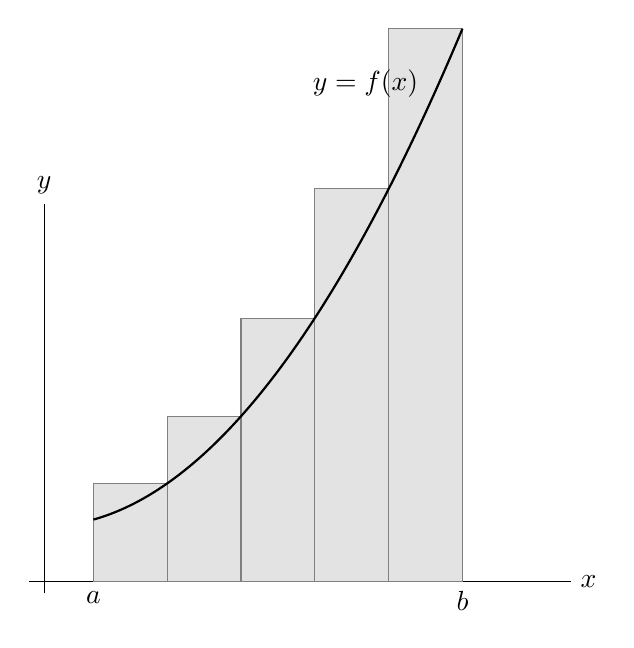
\begin{tikzpicture}[x=1.25cm,y=1.0cm]
  % ejes sin puntas de flecha para evitar conflictos con babel-spanish
  \draw (-0.15,0)--(5.35,0);
  \draw (0,-0.15)--(0,4.8);
  \node[right] at (5.35,0) {$x$};
  \node[above] at (0,4.8) {$y$};

  % rectángulos de Riemann (extremos derechos)
  \fill[gray!22] (0.5,0) rectangle (1.25,{0.35*1.25*1.25+0.7});
  \fill[gray!22] (1.25,0) rectangle (2.0,{0.35*2.0*2.0+0.7});
  \fill[gray!22] (2.0,0) rectangle (2.75,{0.35*2.75*2.75+0.7});
  \fill[gray!22] (2.75,0) rectangle (3.5,{0.35*3.5*3.5+0.7});
  \fill[gray!22] (3.5,0) rectangle (4.25,{0.35*4.25*4.25+0.7});

  \draw[gray] (0.5,0) rectangle (1.25,{0.35*1.25*1.25+0.7});
  \draw[gray] (1.25,0) rectangle (2.0,{0.35*2.0*2.0+0.7});
  \draw[gray] (2.0,0) rectangle (2.75,{0.35*2.75*2.75+0.7});
  \draw[gray] (2.75,0) rectangle (3.5,{0.35*3.5*3.5+0.7});
  \draw[gray] (3.5,0) rectangle (4.25,{0.35*4.25*4.25+0.7});

  % curva
  \draw[thick] plot[domain=.5:4.25,samples=120] (\x,{0.35*\x*\x+0.7});

  \node[below] at (.5,0) {$a$};
  \node[below] at (4.25,0) {$b$};
  \node[above left] at (3.9,{0.35*3.9*3.9+0.7}) {$y=f(x)$};
\end{tikzpicture}
\caption{Aproximación mediante una suma de Riemann. Al refinar la partición, los rectángulos se adaptan cada vez mejor a la región bajo la curva.}
\label{fig:riemann}
\end{figure}

La aproximación mejora cuando todos los subintervalos son pequeños. Para medir su tamaño utilizamos la \emph{norma} o \emph{malla} de la partición,
\[
\|P\|=\max_{1\leq i\leq n}\Delta x_i.
\]
Decir que $\|P\|\to0$ significa que el mayor de los subintervalos de la partición tiende a tener longitud cero. En ese proceso, el número de rectángulos aumenta y sus anchuras disminuyen.

Lo importante es que, si $f$ es continua, las sumas de Riemann se aproximan a un mismo número independientemente de los puntos $c_i$ elegidos dentro de cada subintervalo.

\begin{definition}[Integral definida]
Sea $f:[a,b]\to\R$. Decimos que $f$ es \emph{integrable} en $[a,b]$ si existe un número real $I$ tal que
\[
\sum_{i=1}^{n}f(c_i)\Delta x_i\longrightarrow I
\qquad\text{cuando}\qquad
\|P\|\longrightarrow0,
\]
para cualquier elección de los puntos $c_i\in[x_{i-1},x_i]$. En ese caso escribimos
\[
\boxed{I=\int_a^b f(x)\,dx}
\]
y llamamos a $I$ \emph{integral definida} de $f$ entre $a$ y $b$.
\end{definition}

Toda función continua en un intervalo cerrado es integrable en él. Cuando $f\geq0$, la definición anterior formaliza la intuición geométrica: la integral es el límite de las áreas de los rectángulos utilizados para aproximar la región bajo la gráfica. Cuando $f$ toma valores negativos, los términos correspondientes de la suma de Riemann son negativos; por ello, la integral representa \emph{área con signo}, no necesariamente área geométrica.

\begin{example}
Consideremos $f(x)=x$ en $[0,1]$ y dividamos el intervalo en $n$ partes iguales. Si tomamos como $c_i$ el extremo derecho de cada subintervalo, entonces
\[
\Delta x=\frac1n,
\qquad
c_i=\frac{i}{n}.
\]
La suma de Riemann es
\[
S_n=\sum_{i=1}^{n}\frac{i}{n}\frac1n
=\frac{1}{n^2}\sum_{i=1}^{n}i
=\frac{1}{n^2}\frac{n(n+1)}{2}
=\frac{n+1}{2n}.
\]
Por tanto,
\[
\int_0^1 x\,dx
=\lim_{n\to\infty}S_n
=\frac12.
\]
Geométricamente, este valor coincide con el área del triángulo de base $1$ y altura $1$.
\end{example}

\subsection{Por qué la integral representa el área bajo una curva}

La definición mediante sumas de Riemann permite aproximar el área mediante rectángulos. Sin embargo, existe otra forma de entender la relación entre integral y área que conecta directamente este capítulo con el cálculo diferencial.

Supongamos, en primer lugar, que $f:[a,b]\to\R$ es continua y positiva. Para cada $t\in[a,b]$, definimos
\[
A(t)=\text{área comprendida bajo la gráfica de $f$ entre $a$ y $t$}.
\]
Así, $A(a)=0$ y el área total que queremos calcular es $A(b)$.


Aumentemos ahora $t$ una pequeña cantidad positiva $\Delta t$. Entonces
\[
A(t+\Delta t)-A(t)
\]
es el área de la estrecha región situada bajo la curva entre $t$ y $t+\Delta t$.

Si, para fijar ideas, $f$ es creciente en ese pequeño intervalo, dicha región queda comprendida entre dos rectángulos de base $\Delta t$: uno de altura $f(t)$ y otro de altura $f(t+\Delta t)$. Por tanto,
\[
f(t)\,\Delta t
\leq
A(t+\Delta t)-A(t)
\leq
f(t+\Delta t)\,\Delta t.
\]
Al dividir entre $\Delta t>0$, obtenemos
\[
f(t)
\leq
\frac{A(t+\Delta t)-A(t)}{\Delta t}
\leq
f(t+\Delta t).
\]

\begin{figure}[htbp]
\centering
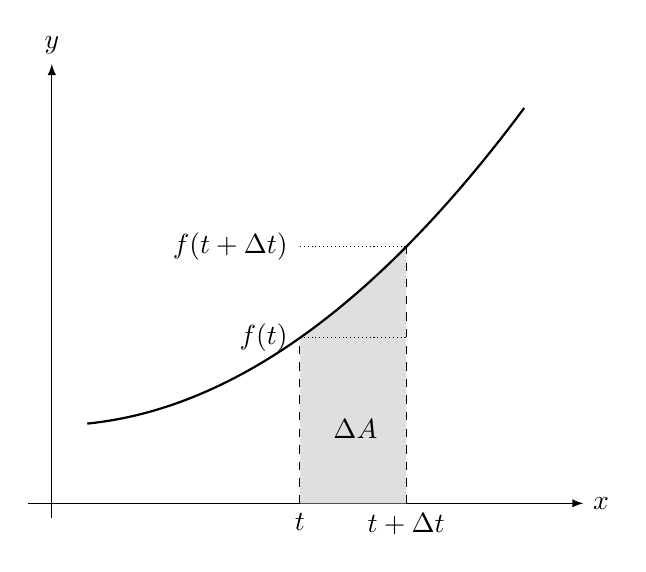
\begin{tikzpicture}[x=1.5cm,y=.9cm]
  \draw[-latex] (-.2,0)--(4.5,0) node[right] {$x$};
  \draw[-latex] (0,-.2)--(0,6.2) node[above] {$y$};
  \fill[gray!25] (2.1,0) -- plot[domain=2.1:3.0,samples=50] (\x,{0.28*\x*\x+1.1}) -- (3.0,0) -- cycle;
  \draw[thick] plot[domain=.3:4,samples=100] (\x,{0.28*\x*\x+1.1});
  \draw[dashed] (2.1,0)--(2.1,{0.28*2.1*2.1+1.1});
  \draw[dashed] (3.0,0)--(3.0,{0.28*3.0*3.0+1.1});
  \draw[densely dotted] (2.1,{0.28*2.1*2.1+1.1}) -- (3.0,{0.28*2.1*2.1+1.1});
  \draw[densely dotted] (2.1,{0.28*3.0*3.0+1.1}) -- (3.0,{0.28*3.0*3.0+1.1});
  \node[below] at (2.1,0) {$t$};
  \node[below] at (3.0,0) {$t+\Delta t$};
  \node at (2.57,1.05) {$\Delta A$};
  \node[left] at (2.08,{0.28*2.1*2.1+1.1}) {$f(t)$};
  \node[left] at (2.08,{0.28*3.0*3.0+1.1}) {$f(t+\Delta t)$};
\end{tikzpicture}
\caption{El incremento de área $\Delta A=A(t+\Delta t)-A(t)$ queda acotado mediante rectángulos.}
\label{fig:incremento-area}
\end{figure}

Como $f$ es continua,
\[
\lim_{\Delta t\to0}f(t+\Delta t)=f(t).
\]
Por el teorema del sándwich,
\[
\lim_{\Delta t\to0}
\frac{A(t+\Delta t)-A(t)}{\Delta t}
=f(t).
\]
Pero el límite de la izquierda es, precisamente, la derivada de $A$. Por tanto,
\[
\boxed{A'(t)=f(t).}
\]

Hemos obtenido una conclusión fundamental: \emph{la función que mide el área acumulada bajo una curva tiene como derivada la propia función que determina la altura de la curva}. En consecuencia, $A$ es una primitiva de $f$.

Si $F$ es cualquier primitiva de $f$, entonces
\[
A(t)=F(t)+C.
\]
Como $A(a)=0$, se tiene
\[
0=F(a)+C,
\qquad\text{de donde}\qquad
C=-F(a).
\]
Así,
\[
A(t)=F(t)-F(a),
\]
y, tomando $t=b$,
\[
\boxed{A(b)=F(b)-F(a).}
\]

Este razonamiento explica por qué, cuando $f\geq0$,
\[
\boxed{\text{área bajo la gráfica de $f$ en $[a,b]$}=\int_a^b f(x)\,dx.}
\]
No se trata simplemente de una fórmula para calcular áreas: la relación surge porque la tasa instantánea de crecimiento del área acumulada es la altura $f(t)$ de la curva.

La hipótesis de monotonía utilizada en el argumento anterior solo simplifica la representación geométrica. Si $f$ es continua pero no monótona, en cada pequeño intervalo $[t,t+\Delta t]$ podemos considerar sus valores mínimo y máximo, $m_{\Delta t}$ y $M_{\Delta t}$. Entonces
\[
m_{\Delta t}\,\Delta t
\leq
A(t+\Delta t)-A(t)
\leq
M_{\Delta t}\,\Delta t.
\]
Por continuidad, tanto $m_{\Delta t}$ como $M_{\Delta t}$ tienden a $f(t)$ cuando $\Delta t\to0$, y se obtiene de nuevo $A'(t)=f(t)$.

Esta idea anticipa el Teorema Fundamental del Cálculo, que formaliza la relación entre derivación, acumulación e integración.

Una integral definida es un número. No debe confundirse con la integral indefinida, que representa una familia de primitivas.

Las propiedades fundamentales son:
\[
\int_a^a f(x)\,dx=0,
\qquad
\int_b^a f(x)\,dx=-\int_a^b f(x)\,dx,
\]
\[
\int_a^b f(x)\,dx
=
\int_a^c f(x)\,dx+\int_c^b f(x)\,dx,
\qquad c\in[a,b],
\]
\[
\int_a^b(\alpha f+\beta g)\,dx
=
\alpha\int_a^b f\,dx+\beta\int_a^b g\,dx.
\]
Además, si $f(x)\leq g(x)$ para todo $x\in[a,b]$, entonces
\[
\int_a^b f(x)\,dx\leq\int_a^b g(x)\,dx.
\]
En particular, si $f\geq0$,
\[
\int_a^b f(x)\,dx\geq0.
\]

La integral es una \emph{acumulación con signo}. Las partes de la gráfica situadas sobre el eje $OX$ contribuyen positivamente y las situadas bajo el eje contribuyen negativamente.

\begin{example}
Sea
\[
f(x)=x-1
\]
en $[0,3]$. Entonces
\[
\int_0^3(x-1)\,dx
=
\left[\frac{x^2}{2}-x\right]_0^3
=\frac32.
\]
Este valor no es el área geométrica total entre la gráfica y el eje $OX$, porque $f<0$ en $[0,1]$. El área geométrica es
\[
\int_0^1(1-x)\,dx+\int_1^3(x-1)\,dx
=\frac12+2=\frac52.
\]
\end{example}

\subsection{Teorema Fundamental y funciones de acumulación}

La conexión entre derivación e integración queda expresada por el Teorema Fundamental del Cálculo.

\begin{theorem}[Teorema Fundamental del Cálculo]
Sea $f$ continua en $[a,b]$ y definamos
\[
F(x)=\int_a^x f(t)\,dt.
\]
Entonces $F$ es derivable en $(a,b)$ y
\[
\boxed{F'(x)=f(x).}
\]
\end{theorem}

La función $F$ mide la acumulación de $f$ desde el punto fijo $a$ hasta el punto variable $x$. El teorema afirma que la tasa instantánea de crecimiento de esa acumulación es precisamente el valor que se está acumulando.

Esta relación permite pasar de un registro a otro:

\begin{center}
\begin{tabular}{p{.27\textwidth}p{.30\textwidth}p{.32\textwidth}}
\toprule
Información sobre $f$ & Información sobre $F(x)=\int_a^x f(t)\,dt$ & Lectura verbal \\
\midrule
$f(x)>0$ & $F'(x)>0$ & la acumulación aumenta \\
$f(x)<0$ & $F'(x)<0$ & la acumulación disminuye \\
$f(x)=0$ & $F'(x)=0$ & $F$ tiene un punto estacionario \\
$f$ creciente & $F''=f'>0$ & la pendiente de $F$ aumenta \\
$f$ decreciente & $F''=f'<0$ & la pendiente de $F$ disminuye \\
\bottomrule
\end{tabular}
\end{center}

Por tanto, una gráfica de $f$ contiene información directa sobre la forma de cualquier función de acumulación asociada, incluso sin calcular explícitamente la integral.

\begin{solvedexercise}
Sea
\[
f(t)=t^2-1
\]
y
\[
F(x)=\int_0^x(t^2-1)\,dt.
\]
Sin calcular inicialmente una fórmula para $F$, determinar sus intervalos de crecimiento y decrecimiento y sus extremos relativos. Después obtener $F$ analíticamente y comprobar las conclusiones.
\tcblower
\textbf{Resolución.}\par\smallskip
Por el Teorema Fundamental,
\[
F'(x)=f(x)=x^2-1.
\]
Así,
\[
F'(x)>0\quad\text{si}\quad x<-1\ \text{o}\ x>1,
\]
y
\[
F'(x)<0\quad\text{si}\quad -1<x<1.
\]
Por tanto, $F$ crece en $(-\infty,-1)$ y $(1,\infty)$ y decrece en $(-1,1)$. En $x=-1$ pasa de crecer a decrecer, luego hay un máximo relativo; en $x=1$ pasa de decrecer a crecer, luego hay un mínimo relativo.

Ahora calculamos
\[
F(x)=\int_0^x(t^2-1)\,dt
=
\left[\frac{t^3}{3}-t\right]_0^x
=
\frac{x^3}{3}-x,
\]
que confirma el análisis anterior. Obsérvese que para estudiar la monotonía de $F$ no era necesario encontrar esta expresión: bastaba estudiar el signo de $f$.
\end{solvedexercise}

La segunda parte del Teorema Fundamental proporciona un procedimiento eficaz para calcular integrales definidas.

\begin{theorem}[Regla de Barrow]
Si $f$ es continua en $[a,b]$ y $G$ es cualquier primitiva de $f$, entonces
\[
\boxed{\int_a^b f(x)\,dx=G(b)-G(a).}
\]
\end{theorem}

Utilizaremos frecuentemente la notación
\[
\left[G(x)\right]_a^b=G(b)-G(a).
\]

\begin{example}
Calcular
\[
\int_1^2(x^2+x+1)\,dx.
\]
Una primitiva es
\[
G(x)=\frac{x^3}{3}+\frac{x^2}{2}+x.
\]
Por tanto,
\[
\int_1^2(x^2+x+1)\,dx
=
\left[\frac{x^3}{3}+\frac{x^2}{2}+x\right]_1^2
=
\frac{29}{6}.
\]
\end{example}

Si el límite superior depende de otra variable, el Teorema Fundamental se combina con la regla de la cadena. Por ejemplo,
\[
F(x)=\int_a^{g(x)}f(t)\,dt
\]
implica
\[
\boxed{F'(x)=f(g(x))g'(x).}
\]
Análogamente,
\[
\frac{d}{dx}\left(\int_{u(x)}^{v(x)}f(t)\,dt\right)
=
f(v(x))v'(x)-f(u(x))u'(x).
\]

\begin{example}
Sea
\[
F(x)=\int_1^{x^2}\ln t\,dt,
\qquad x>0.
\]
Sin calcular la integral,
\[
F'(x)=\ln(x^2)\,2x=4x\ln x.
\]
\end{example}

\subsection{Interpretación de la integral definida}

La misma integral definida representa distintas magnitudes dependiendo de las unidades y del significado de $f$.

Si $f(x)\geq0$, el área entre la gráfica, el eje $OX$ y las rectas $x=a$, $x=b$ es
\[
A=\int_a^b f(x)\,dx.
\]
Si $f$ cambia de signo, el área geométrica total se obtiene integrando $|f|$ o dividiendo el intervalo por los ceros de $f$.

El área comprendida entre dos curvas $y=f(x)$ e $y=g(x)$, con $f\geq g$, es
\[
A=\int_a^b\bigl(f(x)-g(x)\bigr)\,dx.
\]
Si las curvas intercambian su posición, debe localizarse previamente sus puntos de corte y dividir el intervalo.

\begin{solvedexercise}
Calcular el área del recinto limitado por
\[
y=x^2
\qquad\text{y}\qquad
y=2x.
\]
\tcblower
\textbf{Resolución.}\par\smallskip
Los puntos de corte satisfacen
\[
x^2=2x,
\]
de donde $x=0$ y $x=2$. En $(0,2)$ se cumple $2x\geq x^2$. Por tanto,
\[
A=\int_0^2(2x-x^2)\,dx
=
\left[x^2-\frac{x^3}{3}\right]_0^2
=
\boxed{\frac43}.
\]
\end{solvedexercise}

Cuando una magnitud $r(t)$ representa una tasa, la integral
\[
\int_{t_1}^{t_2}r(t)\,dt
\]
representa el cambio neto de la cantidad asociada entre $t_1$ y $t_2$.

\begin{example}[Carga eléctrica]
Si la intensidad que atraviesa un conductor es
\[
I(t)=2+0.5t\qquad (\mathrm{A}),
\]
para $0\leq t\leq10$ s, la carga que atraviesa una sección del conductor durante esos diez segundos es
\[
Q=\int_0^{10}I(t)\,dt
=
\int_0^{10}(2+0.5t)\,dt
=45\ \mathrm{C}.
\]
Las unidades confirman la interpretación:
\[
\mathrm{A}\cdot\mathrm{s}=\mathrm{C}.
\]
\end{example}

Si $v(t)$ es una velocidad, entonces
\[
\int_{t_1}^{t_2}v(t)\,dt
\]
es el \emph{desplazamiento}, mientras que
\[
\int_{t_1}^{t_2}|v(t)|\,dt
\]
es la \emph{distancia total recorrida}. La diferencia entre ambas expresiones refleja el carácter con signo de la integral.

\begin{example}[Trabajo de una fuerza variable]
Una fuerza actúa en la dirección del movimiento y depende del desplazamiento según
\[
F(x)=100+20x\qquad (\mathrm{N}).
\]
El trabajo realizado al mover el punto de aplicación desde $x=0$ hasta $x=3$ m es
\[
W=\int_0^3F(x)\,dx
=
\int_0^3(100+20x)\,dx
=390\ \mathrm{J}.
\]
De nuevo, las unidades son coherentes: $\mathrm{N}\cdot\mathrm{m}=\mathrm{J}$.
\end{example}

El valor medio de una función integrable en $[a,b]$ se define como
\[
\boxed{f_{\mathrm{med}}=\frac1{b-a}\int_a^b f(x)\,dx.}
\]
Si $f$ es continua, existe al menos un punto $c\in[a,b]$ tal que
\[
f(c)=f_{\mathrm{med}}.
\]
Geométricamente, el rectángulo de base $b-a$ y altura $f_{\mathrm{med}}$ tiene la misma área con signo que la región representada por la integral.

También pueden expresarse mediante integrales algunas magnitudes geométricas que aparecen en modelos de diseño. Si $f\geq0$ es suficientemente regular en $[a,b]$, el volumen obtenido al girar la región bajo $y=f(x)$ alrededor del eje $OX$ es
\[
V=\pi\int_a^b f(x)^2\,dx.
\]
La longitud del arco de $y=f(x)$ entre $a$ y $b$ es
\[
L=\int_a^b\sqrt{1+\bigl(f'(x)\bigr)^2}\,dx,
\]
y el área de la superficie generada al girar la curva alrededor del eje $OX$ es
\[
S=2\pi\int_a^b f(x)\sqrt{1+\bigl(f'(x)\bigr)^2}\,dx.
\]
Estas fórmulas muestran cómo una magnitud global se construye sumando contribuciones locales cada vez más pequeñas.

\begin{example}[Volumen de un depósito idealizado]
El perfil de un recipiente de revolución viene dado por
\[
r(x)=\sqrt{1-\frac{x^2}{4}},
\qquad -2\leq x\leq2,
\]
donde $r$ y $x$ se miden en metros. Al girar el perfil alrededor del eje $x$, el volumen es
\[
V=\pi\int_{-2}^2r(x)^2\,dx
=
\pi\int_{-2}^2\left(1-\frac{x^2}{4}\right)dx
=
\frac{8\pi}{3}\ \mathrm{m}^3.
\]
\end{example}

Para comprobar integrales simbólicas con Mathematica utilizaremos principalmente \texttt{Integrate}. Cuando la integral definida no admita una expresión elemental sencilla o interese únicamente un valor numérico, puede emplearse \texttt{NIntegrate}. El objetivo de estas herramientas es comprobar o explorar cálculos, no sustituir la elección razonada del método de integración.

\begin{mathematicacode}
Integrate[x Exp[-x], x]
Integrate[x Exp[-x], {x, 0, 4}]
NIntegrate[Exp[-x^2], {x, 0, 1}]
\end{mathematicacode}

\section{Integrales impropias}
\label{sec:impropias}

La integral definida se ha introducido en intervalos cerrados y para funciones acotadas. En numerosos problemas aparecen intervalos infinitos o funciones que presentan una discontinuidad infinita. Las \emph{integrales impropias} extienden el concepto de integral definida a estas situaciones mediante límites.

\subsection{Intervalos infinitos y singularidades}

\begin{definition}[Integral impropia en un intervalo infinito]
Si $f$ es integrable en todo intervalo $[a,b]$ con $b>a$, se define
\[
\int_a^{\infty}f(x)\,dx
=
\lim_{b\to\infty}\int_a^b f(x)\,dx,
\]
si el límite existe y es finito. En ese caso la integral es \emph{convergente}; en caso contrario es \emph{divergente}.
\end{definition}

Análogamente,
\[
\int_{-\infty}^b f(x)\,dx
=
\lim_{a\to-\infty}\int_a^b f(x)\,dx.
\]
Para una integral sobre toda la recta se elige un punto $c$ y se exige la convergencia de ambas partes:
\[
\int_{-\infty}^{\infty}f(x)\,dx
=
\int_{-\infty}^{c}f(x)\,dx+
\int_c^{\infty}f(x)\,dx.
\]
No es correcto sustituir esta definición por un único límite simétrico, porque podría existir cancelación entre dos divergencias.

\begin{example}
Estudiar
\[
\int_1^{\infty}\frac{1}{x^2}\,dx.
\]
Por definición,
\[
\int_1^{\infty}\frac{1}{x^2}\,dx
=
\lim_{b\to\infty}\left[-\frac1x\right]_1^b
=
\lim_{b\to\infty}\left(1-\frac1b\right)=1.
\]
Por tanto, la integral es convergente.
\end{example}

En cambio,
\[
\int_1^{\infty}\frac1x\,dx
=
\lim_{b\to\infty}\ln b
=\infty,
\]
por lo que diverge. Aunque ambas funciones tienden a cero, lo hacen con distinta rapidez. Que el integrando tienda a cero es necesario para la convergencia en muchas situaciones, pero no es suficiente.

Un resultado básico es
\[
\boxed{\int_1^{\infty}\frac{1}{x^p}\,dx
\text{ converge si y sólo si }p>1.}
\]

También puede aparecer una singularidad en un extremo del intervalo.

\begin{definition}[Integral impropia por una singularidad]
Si $f$ no está acotada cuando $x\to a^+$, se define
\[
\int_a^b f(x)\,dx
=
\lim_{c\to a^+}\int_c^b f(x)\,dx,
\]
si el límite existe y es finito.
\end{definition}

Si la singularidad está en un punto interior $c\in(a,b)$, es obligatorio separar la integral:
\[
\int_a^b f(x)\,dx
=
\int_a^c f(x)\,dx+
\int_c^b f(x)\,dx,
\]
y ambas integrales impropias deben converger.

\begin{solvedexercise}
Estudiar la convergencia de
\[
\int_0^1\frac{1}{\sqrt{x}}\,dx.
\]
\tcblower
\textbf{Resolución.}\par\smallskip
La función no está acotada cuando $x\to0^+$. Por definición,
\[
\int_0^1x^{-1/2}\,dx
=
\lim_{a\to0^+}\int_a^1x^{-1/2}\,dx
=
\lim_{a\to0^+}\left[2\sqrt{x}\right]_a^1.
\]
Así,
\[
\int_0^1\frac{1}{\sqrt{x}}\,dx
=
\lim_{a\to0^+}(2-2\sqrt a)=2.
\]
La integral es convergente aunque el integrando tienda a $+\infty$ en el extremo izquierdo.
\end{solvedexercise}

En general,
\[
\boxed{\int_0^1\frac{1}{x^p}\,dx
\text{ converge si y sólo si }p<1.}
\]

Para funciones no negativas, los criterios de comparación permiten decidir la convergencia sin calcular exactamente la integral. Si
\[
0\leq f(x)\leq g(x)
\]
para $x$ suficientemente grande y $\int_a^\infty g$ converge, entonces $\int_a^\infty f$ también converge. Inversamente, si
\[
0\leq g(x)\leq f(x)
\]
y $\int_a^\infty g$ diverge, entonces $\int_a^\infty f$ diverge.

\begin{example}
Para $x\geq1$,
\[
0<\frac{1}{x^2+1}<\frac{1}{x^2}.
\]
Como
\[
\int_1^{\infty}\frac{1}{x^2}\,dx
\]
converge, también converge
\[
\int_1^{\infty}\frac{1}{x^2+1}\,dx.
\]
En este caso puede calcularse además exactamente:
\[
\int_1^{\infty}\frac{1}{x^2+1}\,dx
=
\left[\arctan x\right]_1^{\infty}
=
\frac{\pi}{4}.
\]
\end{example}

Las integrales impropias aparecen, por ejemplo, al modelar procesos que se prolongan indefinidamente. Si una potencia disipada viene dada por
\[
P(t)=P_0e^{-kt},\qquad k>0,
\]
la energía total disipada desde $t=0$ hasta tiempos arbitrariamente grandes es
\[
E=\int_0^{\infty}P_0e^{-kt}\,dt
=\frac{P_0}{k},
\]
que es finita pese a que el proceso idealizado se extiende hasta $t=\infty$.

\section*{Ejercicios propuestos}
\addcontentsline{toc}{section}{Ejercicios propuestos}

\begin{enumerate}

\item Calcular las siguientes integrales inmediatas:
\begin{enumerate}[label=\alph*)]
\item $\displaystyle\int e^{2x}\,dx$;
\item $\displaystyle\int\frac{10\pi}{x}\,dx$;
\item $\displaystyle\int x^{3/2}\,dx$;
\item $\displaystyle\int\left(4-5e^{-3x}-\cos2x+\sin5x\right)dx$;
\item $\displaystyle\int\frac{2e^{0.1x}}{(1+e^{0.1x})^2}\,dx$.
\end{enumerate}

\item Calcular, aplicando un cambio de variable adecuado cuando sea necesario:
\begin{enumerate}[label=\alph*)]
\item $\displaystyle\int(2x+1)e^{x^2+x}\,dx$;
\item $\displaystyle\int x\sqrt{1-x^2}\,dx$;
\item $\displaystyle\int\frac{x}{1-x^4}\,dx$;
\item $\displaystyle\int\frac{dx}{x\sqrt{1-(\ln x)^2}}$;
\item $\displaystyle\int\frac{e^{3x}}{\sqrt{4-e^{6x}}}\,dx$;
\item $\displaystyle\int \sin^5x\cos x\,dx$.
\end{enumerate}

\item Calcular mediante integración por partes:
\begin{enumerate}[label=\alph*)]
\item $\displaystyle\int\ln x\,dx$;
\item $\displaystyle\int xe^{2x}\,dx$;
\item $\displaystyle\int x^2e^{3x}\,dx$;
\item $\displaystyle\int x\sin x\,dx$;
\item $\displaystyle\int x^2\ln x\,dx$;
\item $\displaystyle\int\arctan x\,dx$;
\item $\displaystyle\int x^2\arctan x\,dx$;
\item $\displaystyle\int e^x\cos x\,dx$.
\end{enumerate}

\item Calcular las integrales racionales:
\begin{enumerate}[label=\alph*)]
\item $\displaystyle\int\frac{2x}{(x-2)(x+1)}\,dx$;
\item $\displaystyle\int\frac{2x}{(x-2)(x+1)^2}\,dx$;
\item $\displaystyle\int\frac{5x+10}{x(x+10)}\,dx$;
\item $\displaystyle\int\frac{3x+5}{x^3-x^2-x+1}\,dx$;
\item $\displaystyle\int\frac{x-1}{x^3+x}\,dx$;
\item $\displaystyle\int\frac{2x^3-4x^2-x-3}{x^2-2x-3}\,dx$;
\item $\displaystyle\int\frac{dx}{(1+x^2)^2}$.
\end{enumerate}
En los apartados con factores repetidos, comparar la descomposición completa en fracciones simples con una reducción de Hermite cuando proceda.

\item Calcular:
\begin{enumerate}[label=\alph*)]
\item $\displaystyle\int\cos^2x\,dx$;
\item $\displaystyle\int\sin^5x\,dx$;
\item $\displaystyle\int\cos^3x\,dx$;
\item $\displaystyle\int\sin^4x\,dx$;
\item $\displaystyle\int\sec x\,dx$;
\item $\displaystyle\int\sec^3x\,dx$;
\item $\displaystyle\int\sin^3x\cos^4x\,dx$.
\end{enumerate}

\item Calcular las integrales irracionales:
\begin{enumerate}[label=\alph*)]
\item $\displaystyle\int\sqrt{16-x^2}\,dx$;
\item $\displaystyle\int\sqrt{x^2+4}\,dx$;
\item $\displaystyle\int\sqrt{x^2-25}\,dx$;
\item $\displaystyle\int\frac{dx}{\sqrt{4-x^2}}$;
\item $\displaystyle\int\frac{dx}{\sqrt{x^2-9}}$;
\item $\displaystyle\int\frac{\sqrt{2x+1}}{x+1}\,dx$.
\end{enumerate}

\item Calcular las integrales definidas:
\begin{enumerate}[label=\alph*)]
\item $\displaystyle\int_1^2(x^2+x+1)\,dx$;
\item $\displaystyle\int_0^2e^{3x}\,dx$;
\item $\displaystyle\int_1^2xe^{x^2}\,dx$;
\item $\displaystyle\int_0^1x^{3/2}\,dx$;
\item $\displaystyle\int_{-1}^{1}\frac{x}{1+x^2}\,dx$;
\item $\displaystyle\int_0^1(e^x+e^{-x})\,dx$.
\end{enumerate}
Antes de integrar, aprovechar simetrías cuando sea posible.

\item Calcular el área limitada por la curva
\[
y=x-1,
\]
el eje $OX$ y las rectas $x=0$ y $x=5$. Distinguir entre integral con signo y área geométrica.

\item Calcular el área limitada por las curvas
\[
y=x+2
\qquad\text{y}\qquad
y=4-x^2.
\]
Representar primero la región y determinar analíticamente los puntos de corte.

\item Calcular el área comprendida entre
\[
y=1,\qquad y=x,\qquad y=1-x^2.
\]
Justificar cómo se divide el intervalo de integración.

\item Sea
\[
F(x)=\int_1^x\bigl(\sin^2t+\ln t\bigr)\,dt,
\qquad x>0.
\]
Calcular $F'(x)$ sin obtener previamente una primitiva del integrando.

\item Calcular la derivada de las funciones:
\begin{enumerate}[label=\alph*)]
\item $\displaystyle F(x)=\int_0^{x^2}(1+\cos^2t)\,dt$;
\item $\displaystyle G(x)=\int_{2x}^{x^2}\ln(1+t^2)\,dt$;
\item $\displaystyle H(x)=\int_{\sin x}^{e^x}\frac{dt}{1+t^2}$.
\end{enumerate}

\item Sea
\[
F(x)=\int_0^x(t^3-4t)\,dt.
\]
Sin calcular primero $F$:
\begin{enumerate}[label=\alph*)]
\item determinar los intervalos de crecimiento y decrecimiento de $F$;
\item localizar sus extremos relativos;
\item estudiar la convexidad de $F$;
\item localizar sus puntos de inflexión;
\item realizar un esbozo cualitativo de $F$ sabiendo que $F(0)=0$.
\end{enumerate}
Comprobar después las conclusiones obteniendo una expresión analítica de $F$.

\item Una función continua $f$ satisface: $f(x)>0$ para $x<1$, $f(1)=0$, $f(x)<0$ para $1<x<4$, $f(4)=0$ y $f(x)>0$ para $x>4$. Además, $f$ es creciente hasta $x=2$ y decreciente a partir de $x=2$. Para
\[
F(x)=\int_0^x f(t)\,dt,
\]
traducir esta información a crecimiento, decrecimiento, extremos y convexidad de $F$. Realizar un esbozo compatible de $F$ sin buscar una fórmula para $f$.

\item La velocidad de una partícula es
\[
v(t)=t^2-t-6,
\qquad 0\leq t\leq4.
\]
\begin{enumerate}[label=\alph*)]
\item calcular el desplazamiento durante los cuatro primeros segundos;
\item calcular la distancia total recorrida;
\item explicar por qué los dos resultados son distintos.
\end{enumerate}

\item La intensidad que circula por un dispositivo es
\[
I(t)=5e^{-0.2t}\ \mathrm{A}.
\]
Calcular la carga que atraviesa el dispositivo entre $t=0$ y $t=10$ s. Determinar también la carga total que circularía en el modelo si el proceso se prolongara indefinidamente.

\item En una conducción, el caudal viene dado por
\[
q(t)=20+4\sin\left(\frac{\pi t}{12}\right)
\qquad (\mathrm{m}^3/\mathrm{h}),
\]
durante $0\leq t\leq24$ h. Determinar el volumen total transportado y el caudal medio durante ese día.

\item Una planta química alimenta un reactor con una corriente cuya tasa neta de entrada de masa es
\[
r(t)=3te^{-0.5t}\qquad (\mathrm{kg/min}).
\]
Si inicialmente hay $20$ kg de sustancia en el reactor, obtener la masa $M(t)$ y calcular $M(5)$. Interpretar la constante de integración y las unidades de cada magnitud.

\item La potencia eléctrica suministrada a una resistencia durante un transitorio es
\[
P(t)=120e^{-0.4t}\qquad (\mathrm{W}).
\]
\begin{enumerate}[label=\alph*)]
\item calcular la energía suministrada durante los primeros $10$ s;
\item calcular la energía total que predice el modelo para $t\geq0$;
\item explicar por qué el segundo cálculo conduce de forma natural a una integral impropia.
\end{enumerate}

\item Una fuerza elástica no lineal viene dada por
\[
F(x)=800x+120x^3\qquad (\mathrm{N}),
\]
donde $x$ se mide en metros. Calcular el trabajo necesario para deformar el elemento desde $x=0$ hasta $x=0.1$ m.

\item Un eje de longitud $L=2$ m presenta una densidad lineal variable
\[
\rho(x)=4+x^2\qquad (\mathrm{kg/m}).
\]
Calcular su masa total y su densidad lineal media.

\item El perfil interior de un depósito de revolución está dado por
\[
r(x)=1+\frac{x}{4},
\qquad 0\leq x\leq4,
\]
en metros. Calcular el volumen del depósito idealizado al girar el perfil alrededor de su eje longitudinal.

\item Calcular la longitud del arco de
\[
y=\frac23x^{3/2},
\qquad 0\leq x\leq3.
\]

\item Estudiar la convergencia y, cuando sea posible, calcular el valor de:
\begin{enumerate}[label=\alph*)]
\item $\displaystyle\int_1^{\infty}\frac{dx}{x^2}$;
\item $\displaystyle\int_1^{\infty}\frac{dx}{x}$;
\item $\displaystyle\int_0^1\frac{dx}{\sqrt{x}}$;
\item $\displaystyle\int_0^1\frac{dx}{x^{3/2}}$;
\item $\displaystyle\int_0^{\infty}e^{-2x}\,dx$;
\item $\displaystyle\int_{-\infty}^{\infty}e^{-|x|}\,dx$.
\end{enumerate}

\item Determinar para qué valores de $p\in\R$ convergen:
\begin{enumerate}[label=\alph*)]
\item $\displaystyle\int_1^{\infty}\frac{dx}{x^p}$;
\item $\displaystyle\int_0^1\frac{dx}{x^p}$.
\end{enumerate}
Explicar por qué las condiciones obtenidas son diferentes.

\item Estudiar la convergencia de
\[
\int_1^{\infty}\frac{1}{x^2+x}\,dx
\]
mediante comparación y comprobar después el resultado calculando la integral.

\item Estudiar la integral
\[
\int_{-1}^{2}\frac{dx}{x-1}.
\]
Explicar por qué no es correcto aplicar directamente la regla de Barrow a una primitiva de $1/(x-1)$ en todo el intervalo.

\item Una función $f$ es positiva, continua y decreciente para $x\geq1$, y se sabe que
\[
\frac{1}{2x^2}\leq f(x)\leq\frac{3}{x^2}.
\]
Decidir si $\int_1^\infty f(x)\,dx$ converge y justificar la respuesta sin calcular una primitiva de $f$.

\item \M Seleccionar cuatro integrales de los ejercicios 2--6, resolverlas manualmente y comprobar el resultado mediante \texttt{Integrate}. En cada caso verificar la primitiva derivándola con \texttt{D}. Si Mathematica devuelve una expresión distinta de la obtenida a mano, utilizar \texttt{Simplify} para estudiar si son equivalentes en el dominio considerado.

\item \M Representar con \texttt{Plot} las funciones
\[
f(x)=x-1,
\qquad
g(x)=4-x^2,
\]
en intervalos adecuados y utilizar la gráfica para decidir cómo deben plantearse los ejercicios 8 y 9. Calcular después las áreas con \texttt{Integrate}. La solución entregada debe contener primero el planteamiento analítico de cada integral.

\item \M Para
\[
F(x)=\int_0^x(t^3-4t)\,dt,
\]
obtener una expresión con \texttt{Integrate}, derivarla con \texttt{D} y representar en gráficos separados el integrando y $F$. Relacionar los signos del integrando con la monotonía de $F$ y los cambios de monotonía del integrando con la convexidad de $F$.

\item \M Comparar numéricamente
\[
\int_0^1e^{-x^2}\,dx
\]
mediante \texttt{NIntegrate} con aproximaciones por sumas de rectángulos usando $n=10$, $50$ y $200$ subintervalos. No es necesario introducir nuevos comandos de Mathematica: las sumas pueden calcularse con una tabla preparada por el profesor o de forma manual/semiautomática. Interpretar qué ocurre al aumentar $n$.

\item \M Utilizar \texttt{NIntegrate} para aproximar
\[
\int_0^{\infty}e^{-x^2}\,dx.
\]
Comparar con la aproximación de $\int_0^b e^{-x^2}\,dx$ para $b=1,2,3,4$ y explicar verbalmente el significado de la convergencia observada.

\item (Examen) Calcular
\[
\int\frac{2x^3-4x^2-x-3}{x^2-2x-3}\,dx.
\]

\item (Examen) Calcular
\[
\int x^2\arctan x\,dx.
\]

\item (Examen) Calcular el área del recinto situado en el primer cuadrante y limitado por
\[
y=3x,
\qquad y=\sqrt{x+1},
\qquad y=1-x^2.
\]
Determinar cuidadosamente qué curvas delimitan cada parte del recinto antes de integrar.

\item (Examen) Calcular
\[
\int\frac{x}{\sqrt{4-x^2}}\,dx.
\]

\item (Examen) Sea
\[
f(x)=10+3xe^{-0.2x}.
\]
Calcular el área bajo la curva, el eje $OX$ y las rectas $x=0$ y $x=10$. Justificar previamente que $f(x)$ es positiva en ese intervalo.

\item Una empresa gestiona una reserva inicial de $100$ millones de unidades de material. La tasa de extracción es
\[
R(t)=3te^{-0.6t}
\]
millones de unidades por año, donde $t$ se mide en años desde el inicio del plan.
\begin{enumerate}[label=\alph*)]
\item interpretar $R(2)$ y sus unidades;
\item obtener la cantidad extraída durante los primeros dos años;
\item obtener una expresión para la reserva restante $S(t)$;
\item calcular la cantidad total que extraería el modelo si se mantuviera indefinidamente y discutir si agotaría la reserva.
\end{enumerate}

\end{enumerate}
